\documentclass{llncs}
\usepackage{graphicx}
\usepackage{listings}

\begin{document}

\title{Linked Open Statistical Data API: requirements and design criteria}

\author{xxx ddd \and yyy sss}

\maketitle

\begin{abstract}

\end{abstract}

\section{Introduction}\label{sec:intro}

Recently, many governments, organisations and companies are opening up their data for others to reuse through \textit{Open Data} portals  \cite{Kalampokis:2011:IJWET}. These data can be exploited to create added value services, which can increase transparency, contribute to economic growth and provide social value to citizens \cite{Janssen:2012}.

A major part of open data concerns statistics (e.g. economical and social indicators) \cite{Capadisli:2013}. These data are are often organised in a multidimensional way, where a measured fact is described based on a number of dimensions. In this case, statistical data are compared to data cubes. Thus, we onwards refer to statistical multidimensional data as \textit{data cubes} or just \textit{cubes}.

Linked data has been introduced as a promising paradigm for opening up data because it facilitates data integration on the Web \cite{Bizer:2009}. Concerning statistical data, the RDF data cube (QB) vocabulary enables modelling data cubes as linked data \cite{Cyganiak:2014:W3C}. In this way it facilitates their integration. Data provided using the QB vocabulary can be accessed using the existing machinery of Linked Data. However, skills and tooling for use of Linked Data (e.g. RDF, SPARQL) are less widespread than some other web technologies (e.g. REST, JSON). For example, there are many visualization libraries that consume data in JSON format (e.g D3.js, charts.js), while there are just a few that consume RDF. That's one of the reasons that there are not so many application for linked open statistical data [REF???].

Moreover, many portals that use the QB vocabulary often adopt different publishing practices \cite{KalampokisChallenges}, thus hampering their interoperability. As a result it is not easy to create generic software tools that operate across linked open statistical datasets. Usually, case specific software are created which assume that linked statistical data are published in a specific way. 

In this paper we describe the requirements and design criteria of an API that standardizes the interaction (i.e. input and output) with Linked Open Statistical Data in a way that facilitated the development of generic software. In this way we keep the advantages of linked data (e.g. data integration) but hide all the complexity by supporting developers to use linked statistical data stored in the form of an RDF Data Cube, while assuming minimal knowledge of Linked Data technologies. Moreover, the API offers a uniform way to access the underlying data hiding any data discrepancies, thus enabling the development of generic software tools that operate across datasets. 

\section{Methodology}\label{sec:methodology}

Related work:
\begin{itemize}
\item  OLAP APIs – interaction with multidimensional data (input): Oracle OLAP API [1], Olap4j [2], ++
\item Standardization of outcome: Json-stat, Json-ld, ++
\end{itemize}

Discussion with developers: Workshop, +++

\section{Solution overview}\label{sec:overview}

A large part of statistical data is isolated, meaning that exists in different portals as different datasets. The technology of Linked data and RDF Data Cube vocabulary solves the problem of distributed data sources through their integration, creating interoperable linked statistical data portals. These portals are used for the design and creation of a Linked Open Statistical Data API. 

The architecture of the API is developed in JSON format offering benefits which are not exist until now. The implementation of JSON-API abolishes the need to implement different data access layers for each tool is created. In the traditional architecture data access layers had to be coded separately leading to additional costs. The JSON-API can be installed on top of any RDF repository and offers basic and advanced operations on RDF Data cubes. 

Moreover, using JSON for accessing RDF Stores is an easier way to build software applications. Developers need neither RDF Data Cube vocabulary nor expert programming skills at LOSD. They have full access at LOSD just using JSON, a much more common and understandable programming language. Through SPARQL queries, JSON-API has access at data cubes returning the asked data in the re-used format of JSON. By this way, all LOSD-related programming and its complexity is now hidden.

As figure 1 shows, JSON-API helps developers create custom applications in JSON. Popular   applications are available on web offering data representation and visualization through the re-use of JSON.  



\begin{figure}
  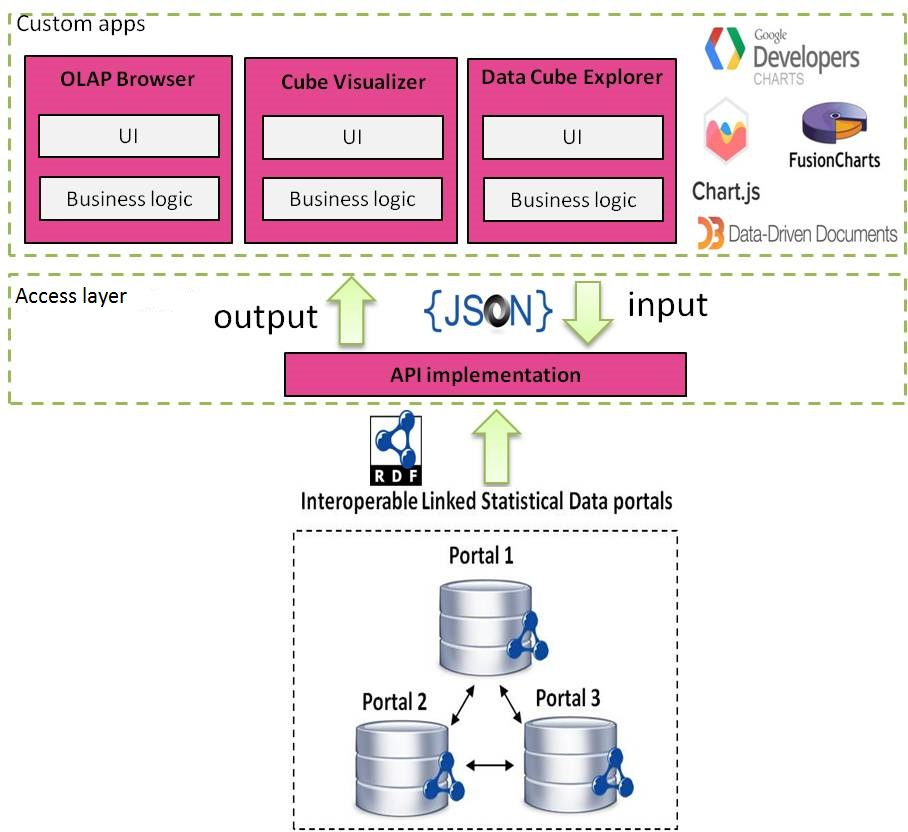
\includegraphics{images/overview.jpg}
\caption{Solution overview}
\label{fig:overview}
\end{figure}


\section{Requirements and design criteria}\label{sec:reqs}

\begin{itemize}
\item need to know what datasets are available
\item need to know about structure to subset the observations
\item in order not to return everything, need to subset
\item don't necessarily need a n-array/ tabular response - array of observations is sufficient. can always get back to the table
\item Filtering
\item Multilinguality
\item Ordering \& paging
\item merging, aggregations
\item json-ld representation is sufficient for query and response format
\item ++
\end{itemize}

API functionality:
\begin{itemize}
\item GET dataset-metadata
\item GET dimensions
\item GET attributes
\item GET measures
\item GET dimension-values
\item GET attribute-values
\item GET dimension-levels
\item GET slice
\item GET table
\item GET cubes
\item GET aggregationSetcubes
\item GET create-aggregations
\item GET cubeOfAggregationSet
\end{itemize}

\cite{Janssen:2012}

possible example for slice/ observation-selection query:
\begin{verbatim} 
{ 
  "jqql:dataset": "scot:home-care-clients",
  "jqql:filter": {
"dimension:gender": "gender:male",
   "dimension:age": { "jqql:greater-than": 50 }
  },
  "jqql:order": {
    "dimension:refPeriod": { "jqql:order-predicate": "ui:sortPriority", "jqql:direction": "jqql:asc"}
  },
  "jqql:page": {
    "jqql:limit": 10,
    "jqql:offset": 0
  }
}
\end{verbatim}

output:
\begin{verbatim} 
{ "observations": [ 
	{ "Average Cost": "1182", 
   	  "Date": "1-1-2013", 
	  "Day": "Tuesday", 
	  "Number of crashes": "5",
	  "Time": "No available time",
      "Total Cost": "5908", 
	  "@id": http://id.mkm.ee/observation/1" }, 
	{ "Average Cost": "400",
	  "Date": "1-1-2013",
	  "Day": "Tuesday",
	  "Number of crashes": "1",
	  "Time": "24:00",
 	  "Total Cost": "400",
	  "@id": "http://id.mkm.ee/observation/2" }
]}
\end{verbatim}

\section{Implementation}\label{sec:impl}

\section{Conclusion}\label{sec:conclusion}


%\begin{acknowledgements}
%If you'd like to thank anyone, place your comments here
%and remove the percent signs.
%\end{acknowledgements}

\bibliographystyle{splncs03}


\bibliography{qbbibfile}   % name your BibTeX data base


\end{document}


